\section{Quantum Lefschetz for quasimaps} \label{Section quasimap mirror theorem}

In \cite{Ga-MF} Gathmann applies his recursion formula for relative stable maps to obtain a new proof of the mirror theorem for hypersurfaces \cite{Givental-mirror} \cite{LLY1}. This can be viewed as a quantum Lefschetz formula, expressing the stable map invariants of $Y$ in terms of those of $X$.

In this section we carry out a similar computation in the quasimap setting, using the recursion found in Theorem \ref{Theorem general recursion} above. We work with generating functions for $2$-pointed quasimap invariants (the minimal number of markings, due to the strong stability condition). The absence of rational tails in the quasimap moduli space makes the recursion much simpler than Gathmann's. We obtain a \emph{quantum Lefschetz theorem for quasimap invariants} (Theorem \ref{Theorem Quantum Lefschetz}); that is, a formula which expresses the quasimap invariants of $Y$ in terms of those of $X$.

Our formula can be viewed as a special case of \cite[Corollary 5.5.1]{CF-K-wallcrossing}, and so can be interpreted as a relation between certain residues of the $\CC^*$-action on spaces of $0$-pointed and $1$-pointed parametrised quasimaps to $Y$. Some of the consequences of this formula are explored in \cite[Section 5.5]{CF-K-wallcrossing}; for instance, it follows in the semipositive case that all primary $\epsilon$-quasimap invariants with a fundamental class insertion can be expressed in terms of $2$-pointed invariants.

\subsection{Setup}
As before, we let $X=X_{\Sigma}$ be a smooth projective toric variety and $i \colon Y \hookrightarrow X$ a smooth very ample hypersurface. We also make the following two assumptions:
\begin{enumerate}
\item \emph{$Y$ semi-positive}: $-K_Y$ is nef;
\item \emph{$Y$ contains all curve classes}: the map $i_* : \Achow_1(Y) \to \Achow_1(X)$ is surjective.
\end{enumerate}
By adjunction, $-K_X$ pairs strictly positively with every curve class coming from $Y$, hence with every curve class by Assumption (2). Thus $-K_X$ is ample; that is, $X$ is Fano\footnote{Kleiman's criterion says that a divisor $D$ is ample if and only if $D \cdot C > 0$ for every curve class $C$ in the closure of the effective cone. But since $X$ is a toric variety the effective cone is finitely generated in $\Achow_1(X)$, hence is closed in $\Achow_1(X)_{\mathbb{R}}$ as it is a finite intersection of half-spaces. So we only need to check $D \cdot C > 0$ for every effective curve class.}. Also note that if $\dim X \geq 3$ then Assumption (2) always holds, due to the Lefschetz hyperplane theorem.

We fix a homogeneous basis $\eta_0, \ldots, \eta_k$ for $\HH^*(X) = \HH^*(X,\QQ)$ and let $\eta^0, \ldots, \eta^k$ denote the dual basis. Without loss of generality we may suppose that $\eta^0=\mathbbm 1_X$ and $\eta^1=Y$. We get an induced basis $\rho_1=i^*\eta_1, \ldots, \rho_k = i^* \eta_k$ for $i^*\HH^*(X)$. Notice that $\rho_0 = i^* \eta_0 = i^* \pt_X = 0$ and $\rho_1 = i^* \eta_1 = \pt_Y$.

We can extend the $\rho_i$ to a basis $\rho_1, \ldots, \rho_l$ for $\HH^*(Y)$ by adding $\rho_{k+1}\ldots,\rho_{l}$. Let $\rho^1, \ldots, \rho^l$ denote the dual basis; notice that $\rho^i$ is \emph{not} equal to $i^* \eta^i$ (they don't even have the same dimension!).

\subsection{Generating functions for quasimap invariants}
As with many results in enumerative geometry, the quantum Lefchetz formula is most naturally stated in terms of generating functions. Here we define several such generating functions for the absolute quasimap invariants of $X$ and $Y$.

We work with two marked points since this is the minimum number required in order for the quasimap space to be nonempty. However since we only take insertions at the first marking we would like to think of these, morally speaking, as $1$-pointed invariants (in Gromov--Witten theory the corresponding statement is literally true, due to the string equation).

For $X$ any smooth projective toric variety\footnote{or any space for which quasimap invariants are defined, for instance a smooth hypersurface in a toric variety} we define: 
\begin{equation*} S_0^X(z,\beta)=(\ev_1)_*\left(\frac{1}{z-\psi_1} \virt{\Q{0}{2}{X}{\beta}}\right) \end{equation*}
for every effective curve class $\beta\in \HH_2^+(X)$. Similarly we define
\begin{equation*} S_0^X(z,q)=\sum_{\beta\geq 0} q^\beta S_0^X(z,\beta)\end{equation*}
where by convention $S_0^X(z,0)= \mathbbm 1_X$. Here $q$ is a formal Novikov variable. These are generating functions for quasimap invariants of $X$ which take values in $\HH^*(X)$.

The same definition applies to $Y$. However, sometimes we may wish to consider only insertions of classes coming from $X$. These are the so-called \emph{restricted quasimap invariants}, and the corresponding generating function is defined as
\begin{equation*} \tilde{S}^Y_0(z,\beta) = (\ev_1)_* \left( \dfrac{1}{z-\psi_1} \virt{\Q{0}{2}{Y}{\beta}} \right) \end{equation*}
where crucially $\ev_1$ is viewed as \emph{mapping to $X$} instead of to $Y$. Thus $\tilde{S}^Y_0(z,\beta)$ takes values in $\HH^*(X)$ and only involves quasimap invariants of $Y$ with insertions from $i^*\HH^*(X)$; on the other hand $S^Y_0(z,\beta)$ takes values in $\HH^*(Y)$ and involves quasimap invariants of $Y$ with arbitrary insertions.

Now, since $X$ and $Y$ are smooth we may use Poincar\'{e} duality to define a push-forward map on cohomology denoted $i_* \colon \HH^k(Y) \to \HH^{k+2}(X)$.

\begin{lemma} $i_* S^Y_0(z,\beta) = \tilde{S}^Y_0(z,\beta)$. \end{lemma}
\begin{proof} This essentially follows by functoriality of cohomological push-forwards and the fact that we have a commuting triangle:
\bcd
\Q{0}{2}{Y}{\beta} \ar[rr,"\ev_1"] \ar[rd,"\ev_1" left=0.2cm] & & Y \ar[ld,"i"] \\
& X & 
\ecd
However we will give a more concrete proof, in order to help familiarise the reader with the generating functions involved. First it is easy to see from the projection formula that:
\begin{align*} i_* \rho^i =
\begin{cases} \eta^i \qquad \text{for $i = 1, \ldots, k$} \\
0 \qquad \text{\ for $i = k+1, \ldots, l$} \end{cases} \end{align*}
%-------------------------------
\begin{comment}We start with the second case. Note that $i^* \HH^*(X) \subseteq \HH^*(Y)$ is a subspace preserved by the non-degenerate Poincar\'{e} pairing, and so we may split $\HH^*(Y)$ into orthogonal subspaces:
\begin{equation*} \HH^*(Y) = i^*\HH^*(X) \oplus i^* \HH^*(X)^\perp \end{equation*}
Here $i^*\HH^*(X)$ is generated by $\rho^1, \ldots, \rho^k$ and $i^*\HH^*(X)^\perp$ is generated by $\rho^{k+1},\ldots,\rho^l$. We claim that $i_* \gamma = 0$ for all $\gamma \in i^*\HH^*(X)^\perp$. We must show that $\langle \delta , i_* \gamma \rangle= 0$ for all $\delta \in \HH^*(X)$. By definition $i_* \gamma$ is the element of $\HH^*(X)$ such that:
\begin{equation*} i_* \gamma \cap [X] = i_* (\gamma \cap [Y]) \end{equation*}
Capping both of these with $\delta$ we obtain
\begin{equation*} (\delta \cup i_* \gamma) \cap [X] = \delta \cap (i_* \gamma \cap [X]) = \delta \cap i_*(\gamma \cap [Y]) = i_*((i^* \delta \cup \gamma) \cap [Y]) \end{equation*}
where the last equality follows from the projection formula. Taking degree zero parts, we see that
\begin{equation*} \langle \delta, i_* \gamma \rangle = \int_X \delta \cup i_* \gamma = \int_Y i^* \delta \cap \gamma = 0 \end{equation*}
where the last equality holds because $\gamma \in i^*\HH^*(X)^\perp$. So indeed $i_* \gamma = 0$ and so $i_* \rho_{k+1} = \ldots = i_* \rho_l = 0$. \end{comment}
%--------------------------------
Now, we can write $S_0^Y(z,\beta)$ as:
\begin{equation*} S_0^Y(z,\beta) = \sum_{i=1}^l \left\langle \dfrac{\ev_1^* \rho_i}{z-\psi_1} \right\rangle_{0,2,\beta}^Y  \rho^i \end{equation*}
Thus applying $i_*$ gives
\begin{align*} i_* S_0^Y(z,\beta)  = \sum_{i=1}^l \left\langle \dfrac{\ev_1^* \rho_i}{z-\psi_1} \right\rangle_{0,2,\beta}^Y   i_* \rho^i
= \sum_{i=1}^k \left\langle \dfrac{\ev_1^* \eta_i}{z-\psi_1} \right\rangle_{0,2,\beta}^Y   \eta^i = \tilde{S}_0^Y(z,\beta) \end{align*}
as claimed. \end{proof}


\subsection{Quantum Lefschetz formula} We now turn to the main result of this section. It gives an equality between generating functions for absolute quasimap invariants of two spaces: those of $X$ on the left-hand-side, and those of $Y$ on the right.
\begin{thm} \label{Theorem Quantum Lefschetz}
Let $X$ and $Y$ be as above. Then
\begin{equation}\label{eqn:mirror}
\dfrac{\sum_{\beta\geq 0} q^\beta\prod_{j=0}^{Y\cdot\beta}(Y+jz)S_0^X(z,\beta)}{P_0(q)}= i_*S_0^Y(z,q)
\end{equation}
where
\begin{align*}
 P_0(q) & = 1 + \sum_{\substack{\beta>0 \\ K_Y\cdot\beta=0}} q^\beta (Y\cdot\beta) \langle \pt_Y,\mathbbm 1_{X}\rangle_{0,(Y\cdot\beta,0),\beta}^{X|Y} \\
& = 1 + \sum_{\substack{\beta>0 \\ K_Y\cdot\beta=0}} q^\beta(Y\cdot\beta)!\langle\psi_1^{Y\cdot\beta-1} \pt_X,\mathbbm 1_{X}\rangle_{0,2,\beta}^X
\end{align*}
\end{thm}

\begin{proof}
Define the following generating function for $2$-pointed relative quasimap invariants:
 \[
  S_{0,(m)}^{X|Y}(z,\beta)=(\ev_1)_*\left(\frac{1}{z-\psi_1}\virt{\Q{0}{(m,0)}{X|Y}{\beta}}\right)
 \]
This coincides with the absolute $S_0^X$-function defined above when $m=0$. Also define the following generating function for ``comb loci invariants'':
\[
 T_{0,(m)}^{X|Y}(z,\beta)=(\ev_1)_*\left(m \virt{\Q{0}{(m,0)}{X|Y}{\beta}}+\frac{1}{z-\psi_1} \virt{\mathcal{D}^{\mathcal{Q}}_{(m,0),1}(X|Y,\beta)} \right)
\]
In the same way as in \cite[Lemma 1.2]{Ga-MF}, it follows from Theorem \ref{Theorem general recursion} that:
\begin{equation}\label{eqn:G}
 (Y+mz) S_{0,(m)}^{X|Y}(z,\beta) = S_{0,(m+1)}^{X|Y}(z,\beta)+ T_{0,(m)}^{X|Y}(z,\beta),
\end{equation}
We can apply this repeatedly to obtain:
\[
 \prod_{j=0}^{Y\cdot\beta}(Y+jz) S_0^X(z,\beta) = \sum_{m=0}^{Y\cdot\beta}\prod_{j=m+1}^{Y\cdot\beta}(Y+jz)T_{0,(m)}^{X|Y}(z,\beta).
\]
We now examine the right-hand-side in detail. $T_{0,(m)}^{X|Y}(z,\beta)$ can be split into two parts: those terms coming from the comb loci and those coming from the relative space.

Let us first consider those coming from the comb loci. Since there are only two markings and the first marking is required to lie on the ``handle'' of the comb, we see from the strong stability condition that there are only two options: a comb with $0$ teeth or a comb with $1$ tooth.

First consider the case of a comb with $0$ teeth. The moduli space is then
\begin{equation*} \Q{0}{2}{Y}{\beta} \end{equation*}
and we require that $Y \cdot \beta = m$. Thus this piece only contributes when 

[UNDER CONSTRUCTION]

the \emph{boundary terms}: since there are only two markings and the first one is required to lie in $Y$, the strong stability condition for quasimaps forces the shape of the source curve to be that of a snake which the hypersurface cuts into two pieces, the internal one of degree $\beta^{(0)}$, and the external one of degree $\beta^{(1)}$ and multiplicity $m^{(1)}$ of contact with $Y$, with the first marked point belonging to the internal component and the second to the external one.

\begin{center}
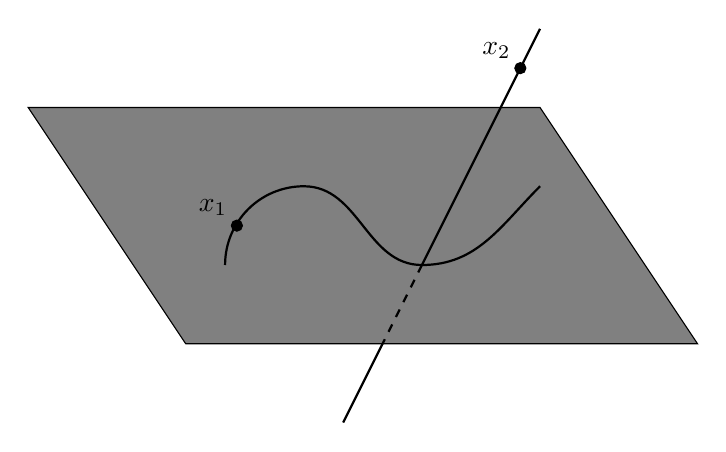
\begin{tikzpicture}
  \draw [fill=gray] (-.5,-1) -- (6,-1) -- (4,2) -- (-2.5,2) -- (-.5,-1);
  \draw [thick] (0,0) to [out=90,in=180] (1,1) to [out=0,in=180] (2.5,0) to [out=0,in=-135] (4,1);
  \draw [thick] (2.5,0) to (4,3);
  \draw [thick,dashed] (2.5,0) to (2,-1);
  \draw [thick] (2,-1) -- (1.5,-2);
  \draw [fill] (3.75,2.5) circle [radius=2pt] node[above left]{$x_2$};
  \draw [fill] (.15,.5) circle [radius=2pt] node[above left]{$x_1$};
 \end{tikzpicture}
\end{center}
 
 The invariants which we need to consider will hence be of the form
 \[
  \langle i^*\eta_i\psi_1^j,\rho^h\rangle_{\Q{0}{2}{Y}{\beta^{(0)}}}\langle \rho_h,\mathbbm 1_{X}\rangle_{\Q{0}{(m^{(1)},0)}{X|Y}{\beta^{(1)}}}, \quad h\in\{1,\ldots,k'\}
 \]
 
 Consider the following dimensional computation:
\begin{align*}
 0\leq \codim \rho^h &= \dim Y-\codim \rho_h \\
 &= \dim Y-\vdim \Q{0}{(m^{(1)},0)}{X|Y}{\beta^{(1)}} \\
 &= \dim Y-(\dim X-3-K_{X}\cdot \beta^{(1)}+2-m^{(1)})\\
 &= K_Y \cdot \beta^{(1)}-Y \cdot \beta^{(1)}+m^{(1)}\leq 0
\end{align*}
 where the last equality follows from adjunction, and the inequality follows from $K_Y\leq 0$ and $m^{(1)}\leq Y \cdot \beta^{(1)}$.
This shows that the only non-trivial contributions are due to the classes $\beta^{(1)}$ such that $K_Y \cdot \beta^{(1)}=0$, and the order of tangency is forced to be maximal, i.e. $m^{(1)}=Y \cdot \beta^{(1)}$. Furthermore, the only relevant insertions are $\rho^1=\mathbbm 1_Y$ and $\rho_1=[pt_Y]$. Finally, $m^{(1)}=Y \cdot \beta^{(1)}$ implies that
\[
 m=\alpha_1=Y \cdot \beta^{(0)}+m^{(1)}=Y \cdot \beta,
\]
hence the boundary contributions do not show up until the very end of the process of ``increasing the multiplicity''.

The remaining term in $T_{(m)}^{X|Y}(z,\beta)$ is $m(\ev_1)_*[\Q{0}{(m,0)}{X|Y}{\beta}]^\text{vir}$; notice that it only gets insertions from the cohomology of $X$ (restricted to $Y$). On the other hand
\[
 \vdim \Q{0}{(m,0)}{X|Y}{\beta}=\dim X-3 -K_X \cdot \beta +2-m \geq r-1
\]
because $m\leq Y\cdot\beta$ and $-(K_X+Y).\beta\geq 0$, by adjunction, projection formula, and for every effective curve class $\beta$ (coming from $Y$, but saying this is superfluous by Lefschetz's hyperplane theorem as we have already remarked); since the restriction of the class $[pt_X]$ to $Y$ vanishes, the only insertion that contributes is $\eta_1$ (by definition of a dual basis, all other dimension 1 classes vanish when restricted to $Y$), forcing the equality $m=Y\cdot\beta$, so that again this correction term is non-trivial only in the last step of the algorithm.

So, in the end, we see that equation \ref{eqn:G} reduces to
\begin{align*}
 &\prod_{j=0}^{Y\cdot\beta}(Y+jz) S_0^X(z,\beta) = T_{(Y\cdot\beta)}^{X|Y}(z,\beta) \\
 &= \sum_{i=1,\ldots,k;j\geq 0}z^{j+1}\eta^i\langle \rho_i\psi_1^j,\mathbbm 1_{Y}\rangle_{\Q{0}{2}{Y}{\beta}} \\
 &+\sum_{\substack{0<\beta^{(0)}<\beta \\ \beta^{(0)}+\beta^{(1)}=\beta}}z^{j+1}\eta^i\langle \rho_i\psi_1^j,\mathbbm 1_{Y}\rangle_{\Q{0}{2}{Y}{\beta^{(0)}}}(Y\cdot\beta^{(1)})\langle [pt_Y],\mathbbm 1_{X}\rangle_{\Q{0}{(Y\cdot\beta^{(1)},0)}{X|Y}{\beta^{(1)}}}\\
 &+\eta^1(Y\cdot\beta)\langle [pt_Y],\mathbbm 1_{X}\rangle_{\Q{0}{(Y\cdot\beta,0)}{X|Y}{\beta}}
\end{align*}
if $\beta$ is such that $K_Y\cdot\beta=0$ (which implies $K_Y\cdot\beta^{(1)}=0$ as well, for every effective decomposition $\beta=\beta^{(0)}+\beta^{(1)}$, due to the semi-positivity assumption on $Y$); while, if $K_Y\cdot\beta<0$, it simply reduces to
\[
 \prod_{j=0}^{Y\cdot\beta}(Y+jz) S_0^X(z,\beta)= \sum_{i=1,\ldots,k;j\geq 0}z^{j+1}\eta^i\langle \rho_i\psi_1^j,\mathbbm 1_{Y}\rangle_{\Q{0}{2}{Y}{\beta}} = i_*S_0^Y(z,\beta).
\]


The proof of the first claim is now evident. We are left with evaluating $P(q)$.

In order to do that, we use again Gathmann's algorithm, this time in the opposite direction, to go all the way back to $X$; so it starts:
\[
 [\Q{0}{(Y \cdot \beta,0)}{X|Y}{\beta}]^\text{vir}=(Y+(Y\cdot\beta-1)\psi_1)[\Q{0}{(Y\cdot\beta-1,0)}{X|Y}{\beta}]^\text{vir}-[D_{Y\cdot\beta}^{\mathcal Q}(X|Y,\beta)]^\text{vir}
\]
When looking at the boundary, the invariants that come into play are of the form
\[
 \langle [pt_Y],\rho^h\rangle_{\Q{0}{2}{Y}{\beta^{(0)}}}\langle \rho_h,\mathbbm 1_{X}\rangle_{\Q{0}{(Y\cdot(\beta-\beta^{(0)})-1,0)}{X|Y}{\beta-\beta^{(0)}}}
\]
but notice that they must vanish by dimensional reasons, since
\[
 \codim(\rho^h)=\dim Y-3+2-K_Y\cdot\beta^{(0)}-\dim Y=-1.
\]
So
\begin{align*}
 & (Y\cdot\beta)\langle [pt_Y],\mathbbm 1_{X}\rangle_{\Q{0}{(Y\cdot\beta,0)}{X|Y}{\beta}} = \\
 & = (Y\cdot\beta)\int_{[\Q{0}{2}{X}{\beta}]^{\text{vir}}}\ev_1^*(\eta_1)\prod_{j=0}^{Y\cdot\beta-1}(\ev_1^*Y+j\psi_1) = \\
 & = (Y\cdot\beta)!\langle[pt_X]\psi_1^{Y\cdot\beta-1},\mathbbm 1_X\rangle_{\Q{0}{2}{X}{\beta}}.
\end{align*}
the second equality because $Y\cdot\eta_1=[pt_X]$ and $Y^2.\eta_1=0$.
\end{proof}

\begin{cor}
 If $Y$ is itself Fano, then there is no correction term
 \[
  \sum_{\beta\geq 0} q^\beta\prod_{j=0}^{Y\cdot\beta}(Y+jz)S_0^X(z,\beta) = i_*S_0^Y(z,q)
 \]
\end{cor}

\begin{cor}
 Let $Y_5$ be the quintic three-fold in $\PP^4$. Then
 \[
  i_*S_0^{Y_5}(z,q)=\frac{I_{\text{small}}^{Y_5}(z,q)}{P^{Y_5}(q)},
 \]
where
\[
 I_{\text{small}}^{Y_5}(z,q)=5H+\sum_{d>0}\frac{\prod_{j=0}^{5d}(H+jz)}{\prod_{j=0}^{d}(H+jz)^5}q^d
\]
and
\[
 P^{Y_5}(q)=1+\sum_{d>0}\frac{(5d)!}{(d!)^5}q^d.
\]
\end{cor}

\begin{remark}
 This formula (and, more generally, formulae for concavex bundles over products of projective spaces) was already obtained in \cite[Theorem 1]{CZ-mirror} via equivariant localisation.
\end{remark}

\subsection{Comparison with the work of Ciocan-Fontanine and Kim}

We would like to compare our formula to \cite[Corollary 5.5.1]{CF-K-wallcrossing}.

In \cite[Section 5]{CF-K-wallcrossing} they introduce (in the more general context of $\epsilon$-stable quasimaps to GIT quotients)
\begin{itemize}
 \item the $J^{\epsilon}$-function:
 \[
  J^\epsilon({\bf t}, z)=\sum_{k\geq 0,\beta\geq 0}q^\beta(\ev_\bullet)_*\left(\frac{\prod_{i=1}^k ev_i^*({\bf t})}{k!}\cap\operatorname{Res}_{F_0}[\QGe{0}{k}{Y}{\beta}]^{\text{vir}}\right)
 \]
\item the $S^\epsilon$-operator
\[
 S^\epsilon(z)(\gamma)=\sum_{m\ge 0,\beta\ge 0}\frac{q^\beta}{m!} 
(ev_1)_*\left(\frac{[\Qe{0}{2+m}{Y}{\beta}]^{\text{vir}}}{z-\psi}ev_2^*(\gamma)\prod_{j=3}^{2+m}ev_j^*({\bf t})\right)
\]
\item the $P^\epsilon$-series
\[
 P^\epsilon({\bf t}, z)=\sum_h\rho^h\sum_{m\geq 0,\beta\geq 0} \frac{q^\beta }{m!}
[\QGe{0}{1+m}{Y}{\beta}]\cap \ev_1^*(\rho_h p_\infty)
\]
where $p_\infty\in H^*_{\Gm}(\PP^1)$ is defined via its restrictions to the $\Gm$-fixed points: $p_{\infty|0}=0,p_{\infty|\infty}=-z$.
\end{itemize}
They prove by localisation that \cite[Theorem 5.4.1]{CF-K-wallcrossing}
\[
 J^\epsilon(z)=S^\epsilon(z)(P^\epsilon).
\]
Furthermore, they prove that, restricting to ${\bf t}=0$ and semi-positive targets, the only class that matches non-trivially with $P^\epsilon_{|{\bf t}=0}$ is $[pt_Y]$, and the above formula takes the simpler form of a product \cite[Corollary 5.5.1]{CF-K-wallcrossing}
\[
 \frac{J^\epsilon |_{{\bf t}=0}}{\langle [pt_Y],  P^\epsilon|_{{\bf t}=0}\rangle}=\mathbbm 1_Y+\sum_h\rho^h(\sum_{\beta\neq 0}q^\beta\langle\frac{\rho_h}{z-\psi},\mathbbm 1_Y\rangle_{0,2,\beta}^\epsilon).
\]
Notice that the restriction of $S^\epsilon(z)(\mathbbm 1_Y)$ to ${\bf t}=0$ that appears on the RHS of this formula coincides with what we have called $S^Y_0(z,q)$ above.

They also observe that, if we write the $\frac{1}{z}$-expansion of $J^{\epsilon}_{{\bf t}=0}$ as
\[
 J^{\epsilon}_{{\bf t}=0}=J^{\epsilon}_{0}(q)\mathbbm 1_Y+O(\frac{1}{z})
\]
then $\langle [pt_Y],  P^\epsilon|_{{\bf t}=0}\rangle=J^{\epsilon}_{0}(q)$.

Let us look more closely at $J^{\epsilon}_{{\bf t}=0}=\sum_{\beta\geq 0}q^\beta(\ev_\bullet)_*\left(\operatorname{Res}_{F_0}[\QGe{0}{0}{Y}{\beta}]^{\text{vir}}\right)$. Recall that in our context $Y\subseteq X$ is a very ample hypersurface and $X$ is toric Fano. Furthermore, set $\epsilon=0^+$. We have the following diagram:

\begin{center}
 \begin{tikzcd}
  \QG{0}{0}{Y}{\beta}\ar[d,hook,"\iota"]\ar[dr,phantom,"\Box"] & F_0^Y\ar[d]\ar[l,hook]\ar[r,"\ev_{\bullet}"] & Y\ar[d,hook,"i"] \\
  \QG{0}{0}{X}{\beta} & F_0^X\ar[l,hook]\ar[r,"\ev_{\bullet}"] & X
 \end{tikzcd}
\end{center}

\begin{itemize}[leftmargin=*]
 \item By a slight generalisation of \cite[Propositions 6.2.2 and 6.2.3]{CFKM}, $\iota_*[\QG{0}{0}{Y}{\beta}]^{\text{vir}}=e(\pi_* E^Y_{0,0,\beta}(z))\cap[\QG{0}{0}{X}{\beta}]^{\text{vir}}$ as $\Gm$-equivariant classes, where $\pi$ is the universal curve on $\QG{0}{0}{X}{\beta}$ and $E^Y_{0,0,\beta}(z)$ is the equivariant line bundle on it associated to $\mathcal O_X(Y)$. This is analagous to the bundle $L_Y$ used in the definition of relative quasimaps (see \S \ref{Subsection relative stable quasimaps}).
\item Since the fibers of $\pi$ are irreducible (by the stability condition and the fact that there are no markings, there can only be the parametrised component), the following splitting holds:
 \[
  e(\pi_* E^Y_{0,0,\beta}(z))=\prod_{j=0}^{Y\cdot\beta} c_1(\sigma_0^* E^Y_{0,0,\beta}(z)\otimes \omega_{\pi}^{\otimes j})
 \]
coming from evaluating at (the $j$-th order infinitesimal thickening of) the zero section $\sigma_0$ and the jet bundles exact sequence:
\begin{center}
 \begin{tikzcd}
  0\ar[r] & \pi_* (E^Y_{0,0,\beta}(-j\sigma_0))\ar[r] & \pi_* E^Y_{0,0,\beta}\ar[r] & \sigma_0^*\operatorname{P}^{j-1}(E^Y_{0,0,\beta}) \ar[r] & 0 \\
  0\ar[r] & \Omega_\pi^{\otimes j}\otimes E^Y_{0,0,\beta}\ar[r] & \operatorname{P}^{j}(E^Y_{0,0,\beta}) \ar[r] & \operatorname{P}^{j-1}(E^Y_{0,0,\beta}) \ar[r] & 0
 \end{tikzcd}
\end{center}
which, restricting to $F_0^X$, gives:
\[
 \iota_*[F_0^Y]^{\text{vir}}=\prod_{j=0}^{Y\cdot\beta}(Y+iz)[F_0^X]^{\text{vir}}.
\]
 \item The small $J^{0^+}$-function for toric varieties has been evaluated by Givental \cite{Givental-equivariantGW}\cite[Definition 7.2.8]{CF-K}:
 \[
  (\ev_{\bullet})_*\frac{[F_0^X]^{\text{vir}}}{e(N_{F_0/\QG{0}{0}{X}{\beta}})}=\prod_{\rho\in\Sigma_X(1)}\frac{\prod_{j=-\infty}^0(D_{\rho}+jz)}{\prod_{j=-\infty}^{\int_{\beta}D_{\rho}}(D_\rho+jz)}=\frac{\prod_{\substack{\rho\in\Sigma_X(1)\colon D_\rho.\beta\leq 0 \\ j=\int_{\beta}D_\rho,\ldots,0}}(D_{\rho}+jz)}{\prod_{\substack{\rho\in\Sigma_X(1)\colon D_\rho.\beta> 0 \\ j=1,\ldots,\int_{\beta}D_\rho}}(D_{\rho}+jz)}
 \]
So, using $\sum_{\rho\in\Sigma_X(1)} D_{\rho}=-K_X$ and $(Y+K_X).\beta=0$, we see that
\[
 J^Y_0(q)=\sum_{\beta\geq 0}q^\beta(Y\cdot\beta)!\frac{\prod_{\rho\in\Sigma_X(1)\colon D_\rho.\beta< 0}(-1)^{-D_{\rho}.\beta}(-D_{\rho}.\beta)!}{\prod_{\rho\in\Sigma_X(1)\colon D_\rho.\beta> 0}(D_{\rho}.\beta)!}
\]
\item Since $X$ is Fano, $J^X_{|{\bf t}=0}=S^X_{|{\bf t}=0}(\mathbbm 1_X)$.
\item The coefficient $\langle[pt_X]\psi_1^{Y\cdot\beta-1},\mathbbm 1_X\rangle_{\Q{0}{2}{X}{\beta}}$ that appears in our $P$-series (multiplied by $(Y\cdot\beta)!$), can be deduced from the expansion of $S^X_{|{\bf t}=0}(\mathbbm 1_X)$ given above, and it turns out to be
\[
 \langle [pt_X],S^X_{|{\bf t}=0}(\mathbbm 1_X)\rangle[z^{Y\cdot\beta}]=\frac{\prod_{\rho\in\Sigma_X(1)\colon D_\rho.\beta< 0}(-1)^{-D_{\rho}.\beta}(-D_{\rho}.\beta)!}{\prod_{\rho\in\Sigma_X(1)\colon D_\rho.\beta> 0}(D_{\rho}.\beta)!}.
\]

\end{itemize}

So we may conclude that the $i_*$ of \cite[Corollary 5.5.1]{CF-K-wallcrossing} coincides with our Equation \ref{eqn:mirror}.